\documentclass[a4paper, 12pt, spanish]{article}

\usepackage[paper=a4paper, left=1.5cm, right=1.5cm, bottom=1.5cm, top=3.5cm]{geometry}
\usepackage[spanish, es-noshorthands]{babel}
\usepackage[utf8x]{inputenc}
\usepackage[none]{hyphenat}
\usepackage[colorlinks,citecolor=black,filecolor=black,linkcolor=black,    urlcolor=black]{hyperref}

% Simbolos matemáticos
\usepackage{amsthm}
\usepackage{amsmath}
\usepackage{amsfonts}
\usepackage{amssymb}
\usepackage[noend]{algpseudocode}
\usepackage{listings}

% Descoración y gráficos
\usepackage{caratulaV}
\usepackage{graphicx} 
\usepackage{fancyhdr}
\usepackage{lastpage}
\usepackage{caption}
\usepackage{subcaption}
\usepackage{multirow}
\usepackage{alltt}
\usepackage{tikz}
\usepackage{color}
\usepackage{verbatim}
\usepackage{framed}

% Bibliografía
\usepackage{natbib}

% Del enunciado
\usepackage{a4wide}
\usepackage{amsmath}
\usepackage{amsfonts}
\usepackage{graphicx}
%\usepackage[ruled,vlined]{algorithm2e}

% Del enunciado
\usepackage{pdfpages}

\newcommand{\kknn}{k}
\newcommand{\kpca}{\alpha}
\newcommand{\kkfold}{K}

% Acomodo fancyhdr.
\pagestyle{fancy}
\thispagestyle{fancy}
\addtolength{\headheight}{1pt}
\lhead{Métodos Númericos}
\rhead{$1^{\mathrm{er}}$ cuatrimestre de 2015}
\cfoot{\thepage /\pageref*{LastPage}}
\renewcommand{\footrulewidth}{0.4pt}

\sloppy

\parskip=5pt % 10pt es el tama de fuente

% Pongo en 0 la distancia extra entre itemes.
\let\olditemize\itemize
\def\itemize{\olditemize\itemsep=0pt}


%\materia{Métodos Númericos}
%\grupo{Conformación del grupo}
%\tituloCaratula{Trabajo Práctico N$^\circ$1\\ \vspace{0.5cm} ``No creo que a él le gustará eso''}


\usepackage{tikz}
%\usepackage{tikz-qtree}


\usetikzlibrary{arrows,backgrounds,calc}

\pgfdeclarelayer{background}
\pgfsetlayers{background,main}

\newcommand{\real}{\mathbb{R}}
\newcommand{\nat}{\mathbb{N}}

\newcommand{\revJ}[1]{{\color{red} #1}}

\newcommand{\convexpath}[2]{
[ 
    create hullnodes/.code={
        \global\edef\namelist{#1}
        \foreach [count=\counter] \nodename in \namelist {
            \global\edef\numberofnodes{\counter}
            \node at (\nodename) [draw=none,name=hullnode\counter] {};
        }
        \node at (hullnode\numberofnodes) [name=hullnode0,draw=none] {};
        \pgfmathtruncatemacro\lastnumber{\numberofnodes+1}
        \node at (hullnode1) [name=hullnode\lastnumber,draw=none] {};
    },
    create hullnodes
]
($(hullnode1)!#2!-90:(hullnode0)$)
\foreach [
    evaluate=\currentnode as \previousnode using \currentnode-1,
    evaluate=\currentnode as \nextnode using \currentnode+1
    ] \currentnode in {1,...,\numberofnodes} {
-- ($(hullnode\currentnode)!#2!-90:(hullnode\previousnode)$)
  let \p1 = ($(hullnode\currentnode)!#2!-90:(hullnode\previousnode) - (hullnode\currentnode)$),
    \n1 = {atan2(\x1,\y1)},
    \p2 = ($(hullnode\currentnode)!#2!90:(hullnode\nextnode) - (hullnode\currentnode)$),
    \n2 = {atan2(\x2,\y2)},
    \n{delta} = {-Mod(\n1-\n2,360)}
  in 
    {arc [start angle=\n1, delta angle=\n{delta}, radius=#2]}
}
-- cycle
}

\newcommand{\todo}[1]{
\textbf{\color{red}{\underline{Nota:} #1}}
}

\newcommand\param[3]{\ensuremath{\mathbf{\textbf{#1}}\,#2\!:} \texttt{#3}}


\newcommand{\degree}{\ensuremath{^\circ}}

\begin{document}
%\setcounter{tocdepth}{2}
\renewcommand{\tablename}{Tabla} 


\thispagestyle{empty}
\materia{Teoría de Lenguajes}
\submateria{Primer Cuatrimestre de 2016}
\titulo{Trabajo Práctico}
\subtitulo{\emph{``SLS: Un simple lenguaje de Scripting''}}
\integrante{Juan Cruz Sosa}{733/12}{nirvguy@gmail.com}
\integrante{Lucas Vuotto}{385/12}{lvuotto@dc.uba.ar}
\integrante{Martín Caravario}{470/12}{martin.caravario@gmail.com}
\maketitle
\newpage
%\begin{titlepage}

%\maketitle

%\end{titlepage}
\setcounter{page}{1}
\newpage
\section{Introducción}

\tableofcontents
\newpage
\section{Gramática}
\label{sec:gramatica}

\subsection{Simbolos Terminales}
	Los símbolos terminales de la gramática son los definidos en el archivo 
	\textit{tokens.py} (Ver sección \ref{codigo:tokens}).

\subsection{Producciones}
	Las producciones de la gramática son las siguientes. Los terminales
	están puestos en negrita y los no terminales en mayúscula.
% TOKENS
\newToken{\COMMENT}{comment}
\newToken{\SEMICOLON}{;}
\newToken{\ID}{id}
\newToken{\NUMBER}{num}
\newToken{\STRING}{str}
\newToken{\TRUE}{true}
\newToken{\FALSE}{false}
\newToken{\RES}{res}
\newToken{\DOT}{.}
\newToken{\LPARENT}{(}
\newToken{\RPARENT}{)}
\newToken{\LBRACKET}{[}
\newToken{\RBRACKET}{]}
\newToken{\LBRACE}{\{}
\newToken{\RBRACE}{\}}
\newToken{\MULTESCALAR}{multiplicacionEscalar}
\newToken{\CAPITALIZAR}{capitalizar}
\newToken{\COLINEALES}{colineales}
\newToken{\PRINT}{print}
\newToken{\LENGTH}{length}
\newToken{\ADD}{+}
\newToken{\MULT}{*}
\newToken{\COMMA}{,}
\newToken{\IF}{if}
\newToken{\ELSE}{else}
\newToken{\WHILE}{while}
\newToken{\FOR}{for}
\newToken{\DO}{do}
\newToken{\SUB}{-}
\newToken{\DIV}{/}
\newToken{\COLON}{:}
\newToken{\RETURN}{return}
\newToken{\LAMBDA}{$\lambda$}
\newToken{\QUESTION}{?}
\newToken{\AND}{AND}
\newToken{\OR}{OR}
\newToken{\NOT}{NOT}
\newToken{\LEQ}{$<=$}
\newToken{\LT}{$<$}
\newToken{\GEQ}{$>=$}
\newToken{\GT}{$>$}
\newToken{\LNOTEQ}{!=}
\newToken{\EQUAL}{==}
\newToken{\MOD}{\%}
\newToken{\POW}{\^}
\newToken{\INC}{++}
\newToken{\DEC}{--}
\newToken{\ADDEQ}{+=}
\newToken{\SUBEQ}{-=}
\newToken{\DIVEQ}{/=}
\newToken{\MULTEQ}{*=}
\newToken{\ASSIGN}{=}


% REGLAS
\subsubsection{Instrucciones}
  \begin{reglas}
	  \regla{INSTRLIST}{INSTAUX}
	  \aregla{INSTAUX INSTRLIST}
    \\	
    \regla{INSTR}{COMMENTLIST}
	  \aregla{INSTROP}
	  \aregla{MAYBECOMMENT}
	  \\
    \regla{COMMENTLIST}{\COMMENT COMMENTLIST}
    \aregla{\LAMBDA}
    \\
    \regla{MAYBECOMMENT}{COMMENT}
    \aregla{\LAMBDA}
    \\
    \regla{INSTROP}{ASSIGN \SEMICOLON}
    \aregla{UNARYMOD \SEMICOLON}
    \aregla{CALL \SEMICOLON}
    \aregla{\RETURN EXPRESSION \SEMICOLON}
    \aregla{LOOP}
    \\
    \regla{INSTROPFOR}{ASSIGN}
    \aregla{ASSIGNEQ}
    \aregla{UNARYMOD}
    \aregla{CALL}
    \aregla{\LAMBDA}
  \end{reglas}

\subsubsection{Bloques de código}
  \begin{reglas}
	  \regla{BLOCK}{INSTR}
	  \aregla{\LBRACE INSTRLIST \RBRACE}
    \\
    \regla{BLOCKAUX}{INSTROP}
	  \aregla{\LBRACE INSTRLIST \RBRACE}
  \end{reglas}

\subsubsection{Condicionales y Ciclos}
  \begin{reglas}
	  \regla{INSTAUX}{MCONDITIONAL}
    \aregla{OCONDITIONAL}
	  \\
    \regla{MCONDITIONAL}{\IF \LPARENT EXPRESSION \RPARENT MCONDITIONAL \ELSE MCONDITIONAL}
    \aregla{BLOCK}
    \\
    \regla{OCONDITIONAL}{\IF \LPARENT EXPRESSION \RPARENT MCONDITIONAL \ELSE OCONDITIONAL}
	  \aregla{\IF \LPARENT EXPRESSION \RPARENT INSTAUX}
    \\
    \regla{LOOP}{\FOR \LPARENT INSTROPFOR \SEMICOLON EXPRESSION \SEMICOLON
    INSTROPFOR \RPARENT BLOCKAUX}
    \aregla{\WHILE \LPARENT EXPRESSION \RPARENT BLOCKAUX}
    \aregla{\DO BLOCK \WHILE \LPARENT EXPRESSION \RPARENT \SEMICOLON}
  \end{reglas}

\subsubsection{Asignaciones y llamadas a funciones}
  \begin{reglas}
	  \regla{ASSIGNOP}{\ADDEQ}
    \aregla{\SUBEQ}
    \aregla{\DIVEQ}
    \aregla{\MULTEQ}
	  \\
	  \regla{ASSIGNEQ}{\ID ASSIGNOP EXPRESSION}
    \aregla{ARRAYMEMBER ASSIGNOP EXPRESSION}
    \aregla{REGISTERMEMBER ASSIGNOP EXPRESSION}
	  \\
    \regla{ASSIGN}{\ID \ASSIGN EXPRESSION}
    \aregla{ARRAYMEMBER \ASSIGN EXPRESSION}
    \aregla{REGISTERMEMBER \ASSIGN EXPRESSION}
	  \\
	  \regla{CALL}{\MULTESCALAR \LPARENT EXPRESSIONLIST \RPARENT}
    \aregla{\CAPITALIZAR \LPARENT EXPRESSIONLIST \RPARENT}
    \aregla{\COLINEALES \LPARENT EXPRESSIONLIST \RPARENT}
    \aregla{\PRINT \LPARENT EXPRESSIONLIST \RPARENT}
    \aregla{\LENGTH \LPARENT EXPRESSIONLIST \RPARENT}
  \end{reglas}

\subsubsection{Términos}
  \begin{reglas}
	  \regla{EXPRESSION}{ARRAY}
	  \aregla{REGISTER}
	  \aregla{LBINARYOP}
	  \aregla{EXPRESSION \QUESTION EXPRESSION \COLON LCOMP}
	  \\
    \regla{EXPRESSIONLIST}{EXPRESSION}
    \aregla{EXPRESSION \COMMA EXPRESSIONLIST} 
  \end{reglas}  

\subsubsection{Arreglos}
  \begin{reglas}
    \regla{ARRAY}{\LBRACKET EXPRESSIONLIST \RBRACKET}
    \\
    \regla{ARRAYMEMBER}{VAR \LBRACKET EXPRESSION \RBRACKET}
    \\
    \regla{REGISTER}{\LBRACE REGISTERLIST \RBRACE}
    \\
    \regla{REGISTERLIST}{\ID \COLON EXPRESSION}
    \aregla{\ID \COLON EXPRESSION \COMMA REGISTERLIST}
    \aregla{\LAMBDA}
    \\ 
    \regla{REGISTERMEMBER}{\ID \DOT \ID}
  \end{reglas}  

\subsubsection{Operaciones Binarias}
  \begin{reglas}
    \regla{LBINARYOP}{EXPRESSION \AND LCOMP}
    \aregla{EXPRESSION \OR LCOMP}
    \aregla{LCOMP}
    \\
    \regla{LCOMP}{LCOMP \LEQ BINARYOP}
    \aregla{LCOMP \GEQ BINARYOP}
    \aregla{LCOMP \LT BINARYOP}
    \aregla{LCOMP \GT BINARYOP}
    \aregla{LCOMP \EQUAL BINARYOP}
    \aregla{LCOMP \LNOTEQ BINARYOP}
    \aregla{BINARYOP}
    \\
    \regla{BINARYOP}{BINARYOP \ADD TERM}
    \aregla{BINARYOP \SUB TERM}
    \aregla{TERM}
    \\
    \regla{TERM}{TERM \MULT UNARYOP}
    \aregla{TERM \DIV UNARYOP}
    \aregla{TERM \MOD UNARYOP}
    \aregla{TERM \POW UNARYOP}
    \aregla{UNARYOP}
  \end{reglas}

\subsubsection{Operaciones Unarias}
  \begin{reglas}
    \regla{UNARYMOD}{\INC VAR}
    \aregla{\DEC VAR}
    \aregla{VAR \INC}
    \aregla{VAR \DEC}
    \\
    \regla{UNARYOP}{\ADD UNARYOP}
    \aregla{\SUB UNARYOP}
    \aregla{\NOT UNARYOP}
    \aregla{UNARYMOD}
    \aregla{FACTOR}
    \\
    \regla{VAR}{\ID}
    \aregla{\RES}
    \aregla{ARRAYMEMBER}
    \aregla{REGISTERMEMBER}
    \\
    \regla{FACTOR}{LITERAL}
    \aregla{VAR}
    \aregla{CALL}
    \aregla{\LPARENT EXPRESSION \RPARENT}
  \end{reglas}

\subsubsection{Literales}
  \begin{reglas}
    \regla{LITERAL}{\NUMBER}
    \aregla{\STRING}
    \aregla{\FALSE}
    \aregla{\TRUE}
  \end{reglas}


\subsection{Expresiones regulares de los tokens}

\begin{tabular}{| c | c | c |}
\hline
Terminal & Token (\textit{lexer\_rules.py}) & Regex \\
\hline
\ & t\_NEWLINE & \textbackslash n+\\
\NUMBER & t\_NUMBER & [0-9]+(\textbackslash.[0-9]+)?\\
\STRING & t\_STRING & \textbackslash[\^ \textbackslash]*\textbackslash\\
\ID & t\_ID & [a-zA-Z][a-zA-Z0-9\_]*\\
\ & t\_ignore\_WHITESPACES & [ \textbackslash t]+\\
\COMMENT & t\_COMMENT & \textbackslash\#.*\\
\SEMICOLON & t\_SEMICOLON & ;\\
\COLON & t\_COLON & :\\
\RBRACE & t\_RBRACE & \}\\
\LBRACE & t\_LBRACE & \{\\
\RBRACKET & t\_RBRACKET & \textbackslash]\\
\LBRACKET & t\_LBRACKET & \textbackslash[\\
\RPARENT & t\_RPARENT & \textbackslash)\\
\LPARENT & t\_LPARENT & \textbackslash(\\
\ADD & t\_ADD & \textbackslash+\\
\ADDEQ & t\_ADDEQ & \textbackslash+=\\
\INC & t\_INC & \textbackslash+\textbackslash+\\
\DEC & t\_DEC & --\\
\ASSIGN & t\_ASSIGN & =\\
\EQUAL & t\_EQUAL & ==\\
\SUB & t\_SUB & -\\
\SUBEQ & t\_SUBEQ & -=\\
\MULT & t\_MULT & \textbackslash*\\
\MULTEQ & t\_MULTEQ & \textbackslash*=\\
\DIV & t\_DIV & /\\
\DIVEQ & t\_DIVEQ & /=\\
\POW & t\_POW & \textbackslash$\hat{ }$ \\
\MOD & t\_MOD & \%\\
\LT & t\_LT & $<$\\
\LEQ & t\_LEQ & $<=$\\
\GEQ & t\_GEQ & $>=$\\
\GT & t\_GT & $>$\\
\LNOTEQ & t\_LNOTEQ & $!=$\\
\QUESTION & t\_QUESTION & \textbackslash?\\
\DOT & t\_DOT & \textbackslash.\\
\COMMA & t\_COMMA & , \\
\hline
\end{tabular}

\subsection{Explicación de la gramática}
La gramática utilizada en trabajo práctico es de tipo LALR(Look-Ahead LR
parser), la cual es un tipo de gramática LR(1) simplificada. Podemos justificar
que nuestra gramática es LALR, debido a que utilizamos la herramienta de
parseo de python PLY. Esta herramienta genera las tablas de parseo utilizando
el algoritmo LALR que usa YACC, y como no se generan conflictos de tipo
shift/reduce ni de tipo reduce/reduce en esa tabla, podemos afirmar que nuestra
gramática es de tipo LALR.

\subsection{Resolución de conflictos}
\begin{enumerate}
    
\item Uno de los conflictos que se nos presentó fue al momento de parsear los
operadores ternarios. Por ejemplo para la entrada: e ? e : e + c, el parser
tenía dos derivaciones posibles. En una asociaba el término de la derecha con
paréntesis de la siguiente forma: e ? e : ( e + c ), y en la otra lo hacia
asociando a izquierda : (e ? e : e) + c. \\
Es por esto que decidimos cambiar nuestra regla: 
\\
\begin{reglas}
  \regla{TERM}{\LPARENT EXPRESSION \RPARENT \QUESTION EXPRESSION \COLON EXPRESSION}
\end{reglas}
\\
Por una de la siguiente forma:
\\
\begin{reglas}
  \regla{TERM}{EXPRESSION \QUESTION EXPRESSION \COLON LCOMP}
\end{reglas}
\\
Esto permitió que el parser utilize como delimitador cada símbolo no terminal
antes de seguir parseando.

\item Otro conflicto que nos presento la gramática fue el llamado Dangling else
  ......

\item Un conflicto de ambiguedad de la gramática que se nos presento fue que
  podiamos derivar en un literal de dos formas distintas, ya sea por EXPRESSION
  --$>$ LITERAL, como por EXPRESSION --$>$ BINARYOP --$>$ FACTOR --$>$ LITERAL. Es por esto que decidimos cambiar la
  gramática agregando la regla FACTOR y quitando la produccion EXPRESSION --$>$
  LITERAL, de la siguiente forma:
  \\
  \\
  \begin{reglas} 
  \regla{FACTOR}{LITERAL}
  \aregla{\LPARENT EXPRESSION \RPARENT}
  \end{reglas}

\item Otro conflicto que tuvimos fue el de la ambiguedad de los operadores
  binarios y sus conflictos de precedencia. Es por eso que decidimos modificar
  nuestra gramática, la cual era:

  \begin{reglas}
    \regla{BINARYOP}{TERM \ADD TERM}
    \aregla{TERM \SUB TERM}
    \aregla{TERM \MULT TERM}
    \aregla{TERM \DIV TERM}
    \aregla{TERM \MOD TERM}
    \aregla{TERM \POW TERM}
    \aregla{TERM \AND TERM}
    \aregla{TERM \OR TERM}
    \aregla{TERM \LT TERM}
    \aregla{TERM \LEQ TERM}
    \aregla{TERM \GEQ TERM}
    \aregla{TERM \EQUAL TERM}
    \aregla{TERM \LNOTEQ TERM}
  \end{reglas}
    \\
    Por una modularizada que separa términos de expresiones y de factores
    permitiendo resolver la ambiguedad presentada, de la siguiente forma:
    \\
  \begin{reglas}
    \regla{BINARYOP}{EXPRESSION \ADD TERM}
    \aregla{EXPRESSION \SUB TERM}
    \aregla{TERM}
    \\
    \regla{TERM}{TERM \MULT FACTOR}
    \aregla{TERM \DIV FACTOR}
    \aregla{TERM \DIV FACTOR}
    \aregla{TERM \DIV FACTOR}
    \aregla{TERM \DIV FACTOR}
    \aregla{TERM \DIV FACTOR}
    \\ 
    \regla{FACTOR}{LITERAL}
    \aregla{\LPARENT EXPRESSION \RPARENT}
  \end{reglas}
\end{enumerate}





\newpage
\section{Pruebas}

\bibliographystyle{plain}
\bibliography{bibliografia}
\newpage
\section{Apendice}

\subsection{Modo de Uso}

\subsection{Código}



\subsection{Enunciado}
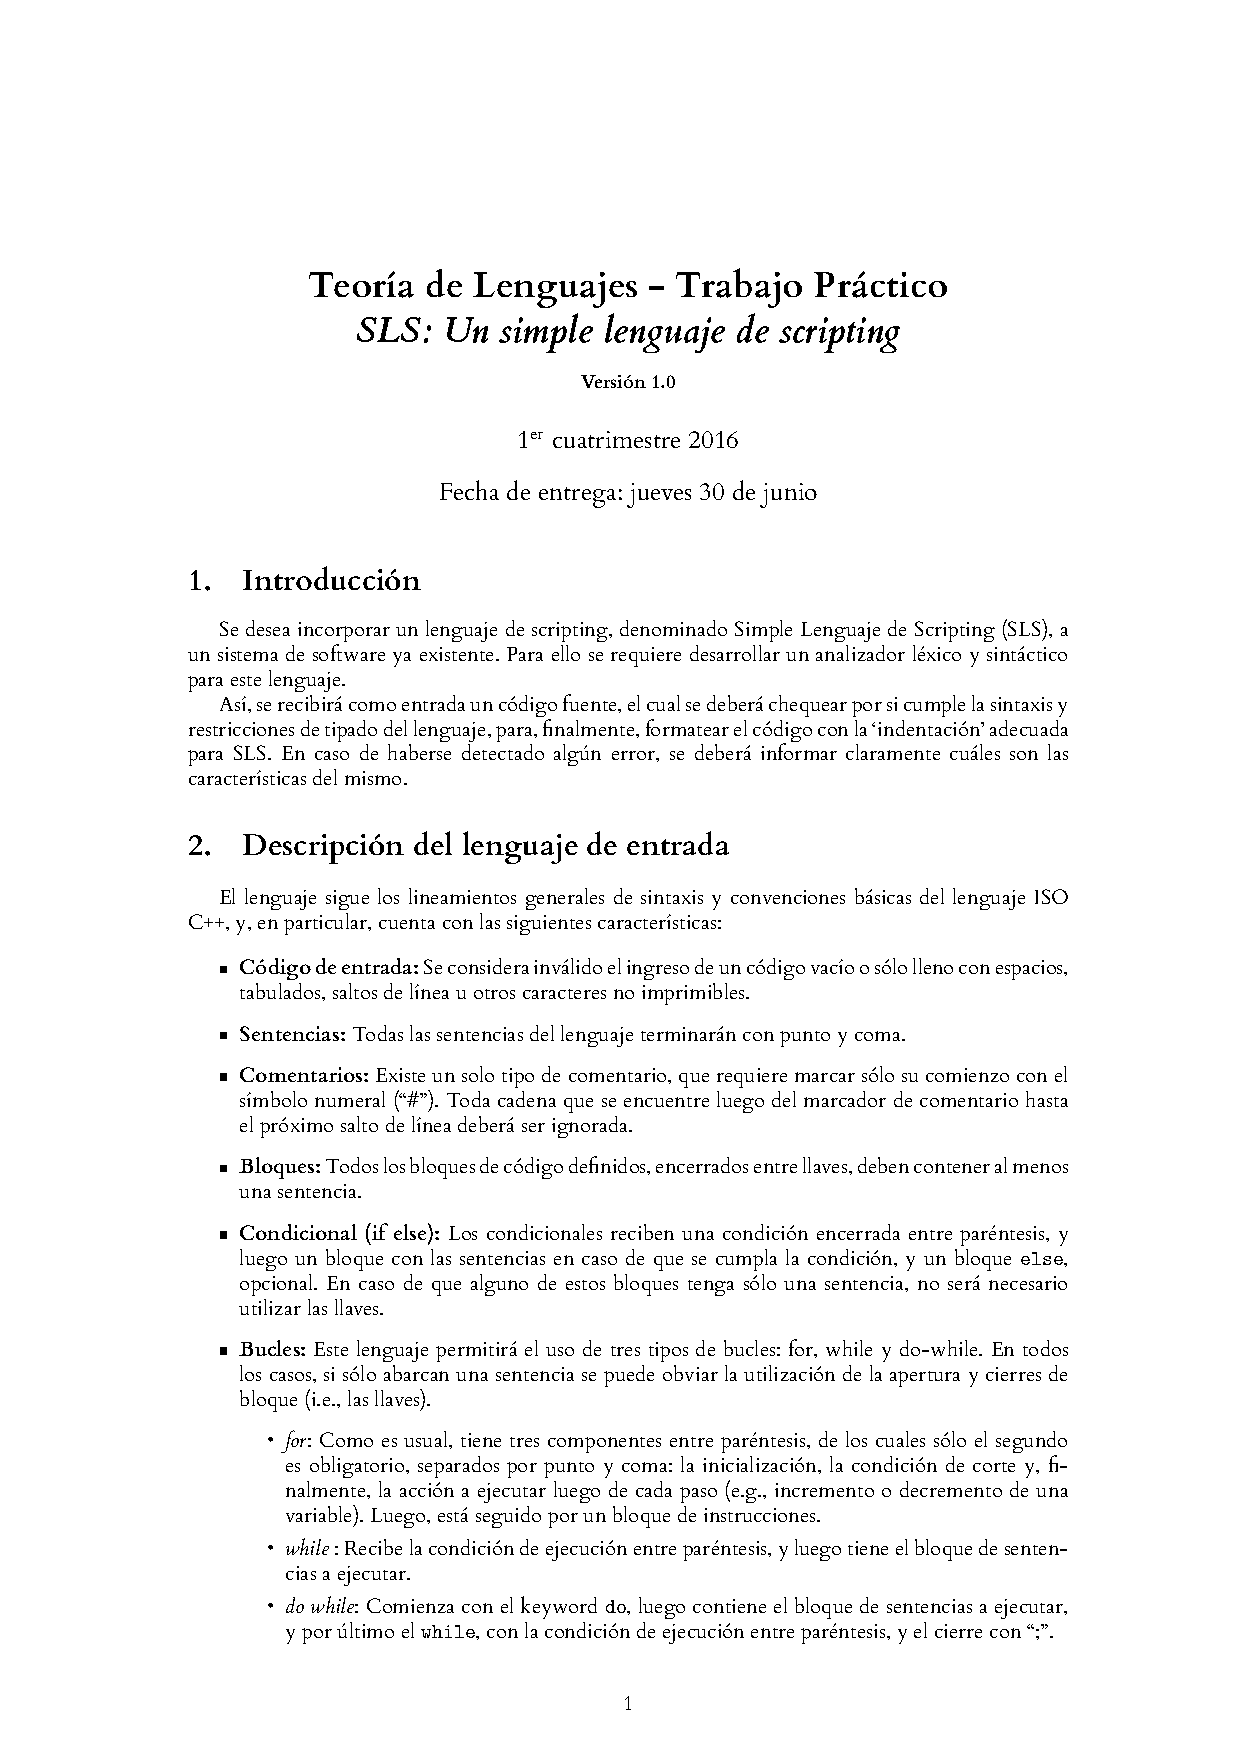
\includepdf[pages=-]{../enunciado/enunciado.pdf}

\ref{LastPage}

\end{document}
